\batchmode
\documentclass{beamer}
\usepackage[utf8]{inputenc}
\usepackage[ngerman]{babel}

\usetheme[deutsch]{KIT}
\author{Jan Haag (jan.haag@student.kit.edu)}
\title{Programmieren Tutorium 3 -- Konventionen, Kontrollstrukturen}
\institute{Institut f\"{u}r Zeritfizierbare und Vertra\"{u}nsw\"{u}rdige Informatiksysteme (ZVI)}
\TitleImage[scale=0.225]{frontpic.jpg}

\begin{document}
\begin{frame}
\maketitle
\end{frame}

\begin{frame}
\frametitle{Inhalt}
\tableofcontents
\end{frame}

\section{Korrektur des \"{U}bungsblattes}
\begin{frame}
\frametitle{Korrektur des \"{U}bungsblattes}
Siehe Code.
\end{frame}

\section{Konventionen}
\begin{frame}
\frametitle{Konventionen}
\begin{itemize}
\item Helfen, code verst\"{a}ndlich zu halten
\item Helfen programmen, die Code analysieren
\pause
\item Sorgen daf\"{u}r, dass andere (auch ihr selbst, in 8 wochen!) nachvollziehen k\"{o}nnen, was der code tut.
\pause
\item \emph{Nichteinhaltung f\"{u}hrt zu Punktabzug!}
\end{itemize}
\end{frame}

\subsection{Namen}
\begin{frame}[fragile]
\frametitle{Namenskonventionen}
\begin{itemize}
\item Namen in CamelCase
\item Klassennamen gross (\verb|class MyClass {...}|)
\item Variablennamen klein, Namen i. d. R. Substantive (\verb|int importantIntVariable;|)
\item Laufvariablen mit einem buchstaben, Namen i. d. R anfangsbuchstabe des
typen oder darauf folgende buchstaben (\verb|for(int i = 0; i < 10; i++) {...}|)
\item Methodennamen klein, Namen i. d. R. Verben (\verb|int doSomething(int foo) {...}|)
\item Methoden zum Lesen oder Schreiben von Attributen hei\ss{}en getAttr bzw. setAttr
\item Konstanten in gro\ss{}buchstaben, w\"{o}rter durch \verb|_|
getrennt (\verb|public static final int IMPORTANT_CONSTANT = 1;|)
\end{itemize}
\end{frame}

\begin{frame}
\frametitle{Dateien und Inhalte}
\begin{itemize}
\item Jede Klasse in eine eigene Datei
\item Dateiname: Klassenname.java
\end{itemize}
\end{frame}

\subsection{Whitespace}
\begin{frame}
\frametitle{Whitespace-Konventionen}
Siehe Dokumentation zu Checkstyle 1.
\end{frame}

\section{Kontrollstrukturen}
\begin{frame}[fragile]
\frametitle{Kontrollstrukturen -- if}
\begin{verbatim}
if (boolean) {
    // code to run if boolean is true
} else {
    // code to run otherwise
}
\end{verbatim}
\end{frame}

\begin{frame}[fragile]
\frametitle{Kontrollstrukturen -- Tern\"{a}rer Operator}
\begin{verbatim}
String s = cond ? "true" : "false";
\end{verbatim}
$\rightarrow$ Nur f\"{u}r kurze Bedingungen und Zweige geeignet!
\end{frame}

\begin{frame}[fragile]
\frametitle{Kontrollstrukturen -- switch}
\begin{verbatim}
switch (var) {
    case 1:
        // code if var is 1
        break;
    case 2:
    case 3:
        // code if var is 2 or 3
        break;
    default:
        // code to run if none of the above conditions hold
        break;
}
\end{verbatim}
\pause
$\rightarrow$ Nur f\"{u}r primitive Datentypen!
\end{frame}

\begin{frame}[fragile]
\frametitle{Kontrollstrukturen -- while}
\begin{verbatim}
while (condition) {
    // code to run while condition holds
}
\end{verbatim}
$\rightarrow$ Die Bedingung wird vor dem Schleifendurchlauf gepr\"{u}ft.
\end{frame}

\begin{frame}[fragile]
\frametitle{Kontrollstrukturen -- do-while}
\begin{verbatim}
do {
    // code to run while condition holds
} while (condition);
\end{verbatim}
$\rightarrow$ Die Bedingung wird nach dem Schleifendurchlauf gepr\"{u}ft.
\end{frame}

\begin{frame}[fragile]
\frametitle{Kontrollstrukturen -- for}
\begin{verbatim}
for (start; stop; step) {
    //code to run while stop condition is not false
}
\end{verbatim}
$\rightarrow$ Z\"{a}hlschleife
\end{frame}

\begin{frame}[fragile]
\frametitle{Kontrollstrukturen -- Schleifenkontrolle}
Nur in ausnahmef\"{a}llen, da verst\"{a}ndlichkeit schnell leidet\\
Schleifenabbruch mit \verb|break;|
\end{frame}


\section{Aufgaben}
\begin{frame}
\frametitle{Aufgabe}
$fak(0)=1$; $fak(n) = n\cdot{}fak(n-1)$
\end{frame}

\begin{frame}
\frametitle{Ende}
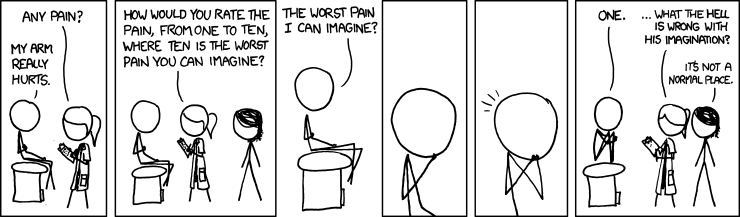
\includegraphics[scale=0.4]{pain_rating.png}
\end{frame}
\end{document}
